% Options for packages loaded elsewhere
\PassOptionsToPackage{unicode}{hyperref}
\PassOptionsToPackage{hyphens}{url}
%
\documentclass[
  12pt, openany]{book}
\usepackage{lmodern}
\usepackage{amssymb,amsmath}
\usepackage{ifxetex,ifluatex}
\ifnum 0\ifxetex 1\fi\ifluatex 1\fi=0 % if pdftex
  \usepackage[T1]{fontenc}
  \usepackage[utf8]{inputenc}
  \usepackage{textcomp} % provide euro and other symbols
\else % if luatex or xetex
  \usepackage{unicode-math}
  \defaultfontfeatures{Scale=MatchLowercase}
  \defaultfontfeatures[\rmfamily]{Ligatures=TeX,Scale=1}
\fi
% Use upquote if available, for straight quotes in verbatim environments
\IfFileExists{upquote.sty}{\usepackage{upquote}}{}
\IfFileExists{microtype.sty}{% use microtype if available
  \usepackage[]{microtype}
  \UseMicrotypeSet[protrusion]{basicmath} % disable protrusion for tt fonts
}{}
\makeatletter
\@ifundefined{KOMAClassName}{% if non-KOMA class
  \IfFileExists{parskip.sty}{%
    \usepackage{parskip}
  }{% else
    \setlength{\parindent}{0pt}
    \setlength{\parskip}{6pt plus 2pt minus 1pt}}
}{% if KOMA class
  \KOMAoptions{parskip=half}}
\makeatother
\usepackage{xcolor}
\IfFileExists{xurl.sty}{\usepackage{xurl}}{} % add URL line breaks if available
\IfFileExists{bookmark.sty}{\usepackage{bookmark}}{\usepackage{hyperref}}
\hypersetup{
  pdftitle={Philosophy in the Wild},
  pdfauthor={George W. Matthews},
  hidelinks,
  pdfcreator={LaTeX via pandoc}}
\urlstyle{same} % disable monospaced font for URLs
\usepackage[margin=2cm]{geometry}
\usepackage{longtable,booktabs}
% Correct order of tables after \paragraph or \subparagraph
\usepackage{etoolbox}
\makeatletter
\patchcmd\longtable{\par}{\if@noskipsec\mbox{}\fi\par}{}{}
\makeatother
% Allow footnotes in longtable head/foot
\IfFileExists{footnotehyper.sty}{\usepackage{footnotehyper}}{\usepackage{footnote}}
\makesavenoteenv{longtable}
\usepackage{graphicx,grffile}
\makeatletter
\def\maxwidth{\ifdim\Gin@nat@width>\linewidth\linewidth\else\Gin@nat@width\fi}
\def\maxheight{\ifdim\Gin@nat@height>\textheight\textheight\else\Gin@nat@height\fi}
\makeatother
% Scale images if necessary, so that they will not overflow the page
% margins by default, and it is still possible to overwrite the defaults
% using explicit options in \includegraphics[width, height, ...]{}
\setkeys{Gin}{width=\maxwidth,height=\maxheight,keepaspectratio}
% Set default figure placement to htbp
\makeatletter
\def\fps@figure{htbp}
\makeatother
\setlength{\emergencystretch}{3em} % prevent overfull lines
\providecommand{\tightlist}{%
  \setlength{\itemsep}{0pt}\setlength{\parskip}{0pt}}
\setcounter{secnumdepth}{5}
\usepackage[Bjornstrup]{fncychap}
\usepackage{cclicenses}
\usepackage{fancyvrb}
\usepackage{booktabs}
\usepackage{longtable}
\usepackage[bf,singlelinecheck=off]{caption}
\usepackage{etoolbox}
\AtBeginEnvironment{centercap}{\scriptsize}
\BeforeBeginEnvironment{epigraph}{\vspace*{2em}}
\usepackage{tcolorbox}

\newsavebox{\FVerbBox}
\newenvironment{FVerbatim}
 {\VerbatimEnvironment
  \begin{center}
  \setlength{\fboxrule}{0pt}
  \begin{lrbox}{\FVerbBox}
  \begin{BVerbatim}}
 {\end{BVerbatim}
  \end{lrbox}
  \fbox{\usebox{\FVerbBox}}
  \end{center}}

%\setmainfont[UprightFeatures={SmallCapsFont=AlegreyaSC-Regular}]{Alegreya}

\usepackage{framed,color}
\definecolor{shadecolor}{RGB}{248,248,248}

\renewcommand{\textfraction}{0.05}
\renewcommand{\topfraction}{0.8}
\renewcommand{\bottomfraction}{0.8}
\renewcommand{\floatpagefraction}{0.75}

%\renewenvironment{quote}{\begin{VF}}{\end{VF}}
\let\oldhref\href
\renewcommand{\href}[2]{#2\footnote{\url{#1}}}

\ifxetex
  \usepackage{letltxmacro}
  \setlength{\XeTeXLinkMargin}{1pt}
  \LetLtxMacro\SavedIncludeGraphics\includegraphics
  \def\includegraphics#1#{% #1 catches optional stuff (star/opt. arg.)
    \IncludeGraphicsAux{#1}%
  }%
  \newcommand*{\IncludeGraphicsAux}[2]{%
    \XeTeXLinkBox{%
      \SavedIncludeGraphics#1{#2}%
    }%
  }%
\fi%

\makeatletter
\newenvironment{kframe}{%
\medskip{}
\setlength{\fboxsep}{.8em}
 \def\at@end@of@kframe{}%
 \ifinner\ifhmode%
  \def\at@end@of@kframe{\end{minipage}}%
  \begin{minipage}{\columnwidth}%
 \fi\fi%
 \def\FrameCommand##1{\hskip\@totalleftmargin \hskip-\fboxsep
 \colorbox{shadecolor}{##1}\hskip-\fboxsep
     % There is no \\@totalrightmargin, so:
     \hskip-\linewidth \hskip-\@totalleftmargin \hskip\columnwidth}%
 \MakeFramed {\advance\hsize-\width
   \@totalleftmargin\z@ \linewidth\hsize
   \@setminipage}}%
 {\par\unskip\endMakeFramed%
 \at@end@of@kframe}
\makeatother

\makeatletter
\@ifundefined{Shaded}{
}{\renewenvironment{Shaded}{\begin{kframe}}{\end{kframe}}}
\makeatother


\newenvironment{rmdblock}[1]
  {
  \begin{itemize}
  \renewcommand{\labelitemi}{
    \raisebox{-.7\height}[0pt][0pt]{
      {\setkeys{Gin}{width=3em,keepaspectratio}\includegraphics{img/#1}}
    }
  }
  \setlength{\fboxsep}{1em}
  \begin{kframe}
  \item
  }
  {
  \end{kframe}
  \end{itemize}
  }
\newenvironment{note}
  {\begin{rmdblock}{note}}
  {\end{rmdblock}}
\newenvironment{caution}
  {\begin{rmdblock}{caution}}
  {\end{rmdblock}}
\newenvironment{important}
  {\begin{rmdblock}{important}}
  {\end{rmdblock}}
\newenvironment{tip}
  {\begin{rmdblock}{tip}}
  {\end{rmdblock}}
\newenvironment{warning}
  {\begin{rmdblock}{warning}}
  {\end{rmdblock}}
\newenvironment{question}
  {\begin{rmdblock}{question}}
  {\end{rmdblock}}
\newenvironment{slides}
  {\begin{rmdblock}{slides}}
  {\end{rmdblock}}

\newenvironment{epigraph}%
{
\begin{flushright}
\begin{minipage}{30em}
\begin{flushright}
\itshape
}%
{
\end{flushright}
\end{minipage}
\end{flushright}
\vspace{1em}
}

\newtcolorbox{argument}{
  colback=black!5!white,
  colframe=black!30,
  coltext=black,
  text width=12cm,
  boxsep=5pt,
  arc=4pt}

\newtcolorbox{example}{
  colback=black!5!white,
  colframe=black!30,
  coltext=black,
  text width=15cm,
  boxsep=5pt,
  arc=4pt}


%\newenvironment{argument}{\par\begin{quote}}{\end{quote}\par}

%\newenvironment{argument}{\par\begin{tcolorbox}}{\end{tcolorbox}\par}

\newenvironment{centerpic}{\begin{center}}{\end{center}}

\newenvironment{centercap}{\begin{center}}{\end{center}}

\newenvironment{embed}{\begin{center}}{\end{center}}

\newenvironment{slideshow}{}

\newenvironment{passage}{\begin{quotation}}{\end{quotation}}

%%%% Suppress title page

\let\oldmaketitle\maketitle
\AtBeginDocument{\let\maketitle\relax}

\title{Philosophy in the Wild}
\usepackage{etoolbox}
\makeatletter
\providecommand{\subtitle}[1]{% add subtitle to \maketitle
  \apptocmd{\@title}{\par {\large #1 \par}}{}{}
}
\makeatother
\subtitle{an introduction}
\author{\textbf{George W. Matthews}}
\date{last revised: 2020-10-19}

\begin{document}
\maketitle

\thispagestyle{empty}
\begin{center}

{\Huge\textbf{Philosophy in the Wild}}



{\Large\textit{an introductiom}}

\vspace*{2em}

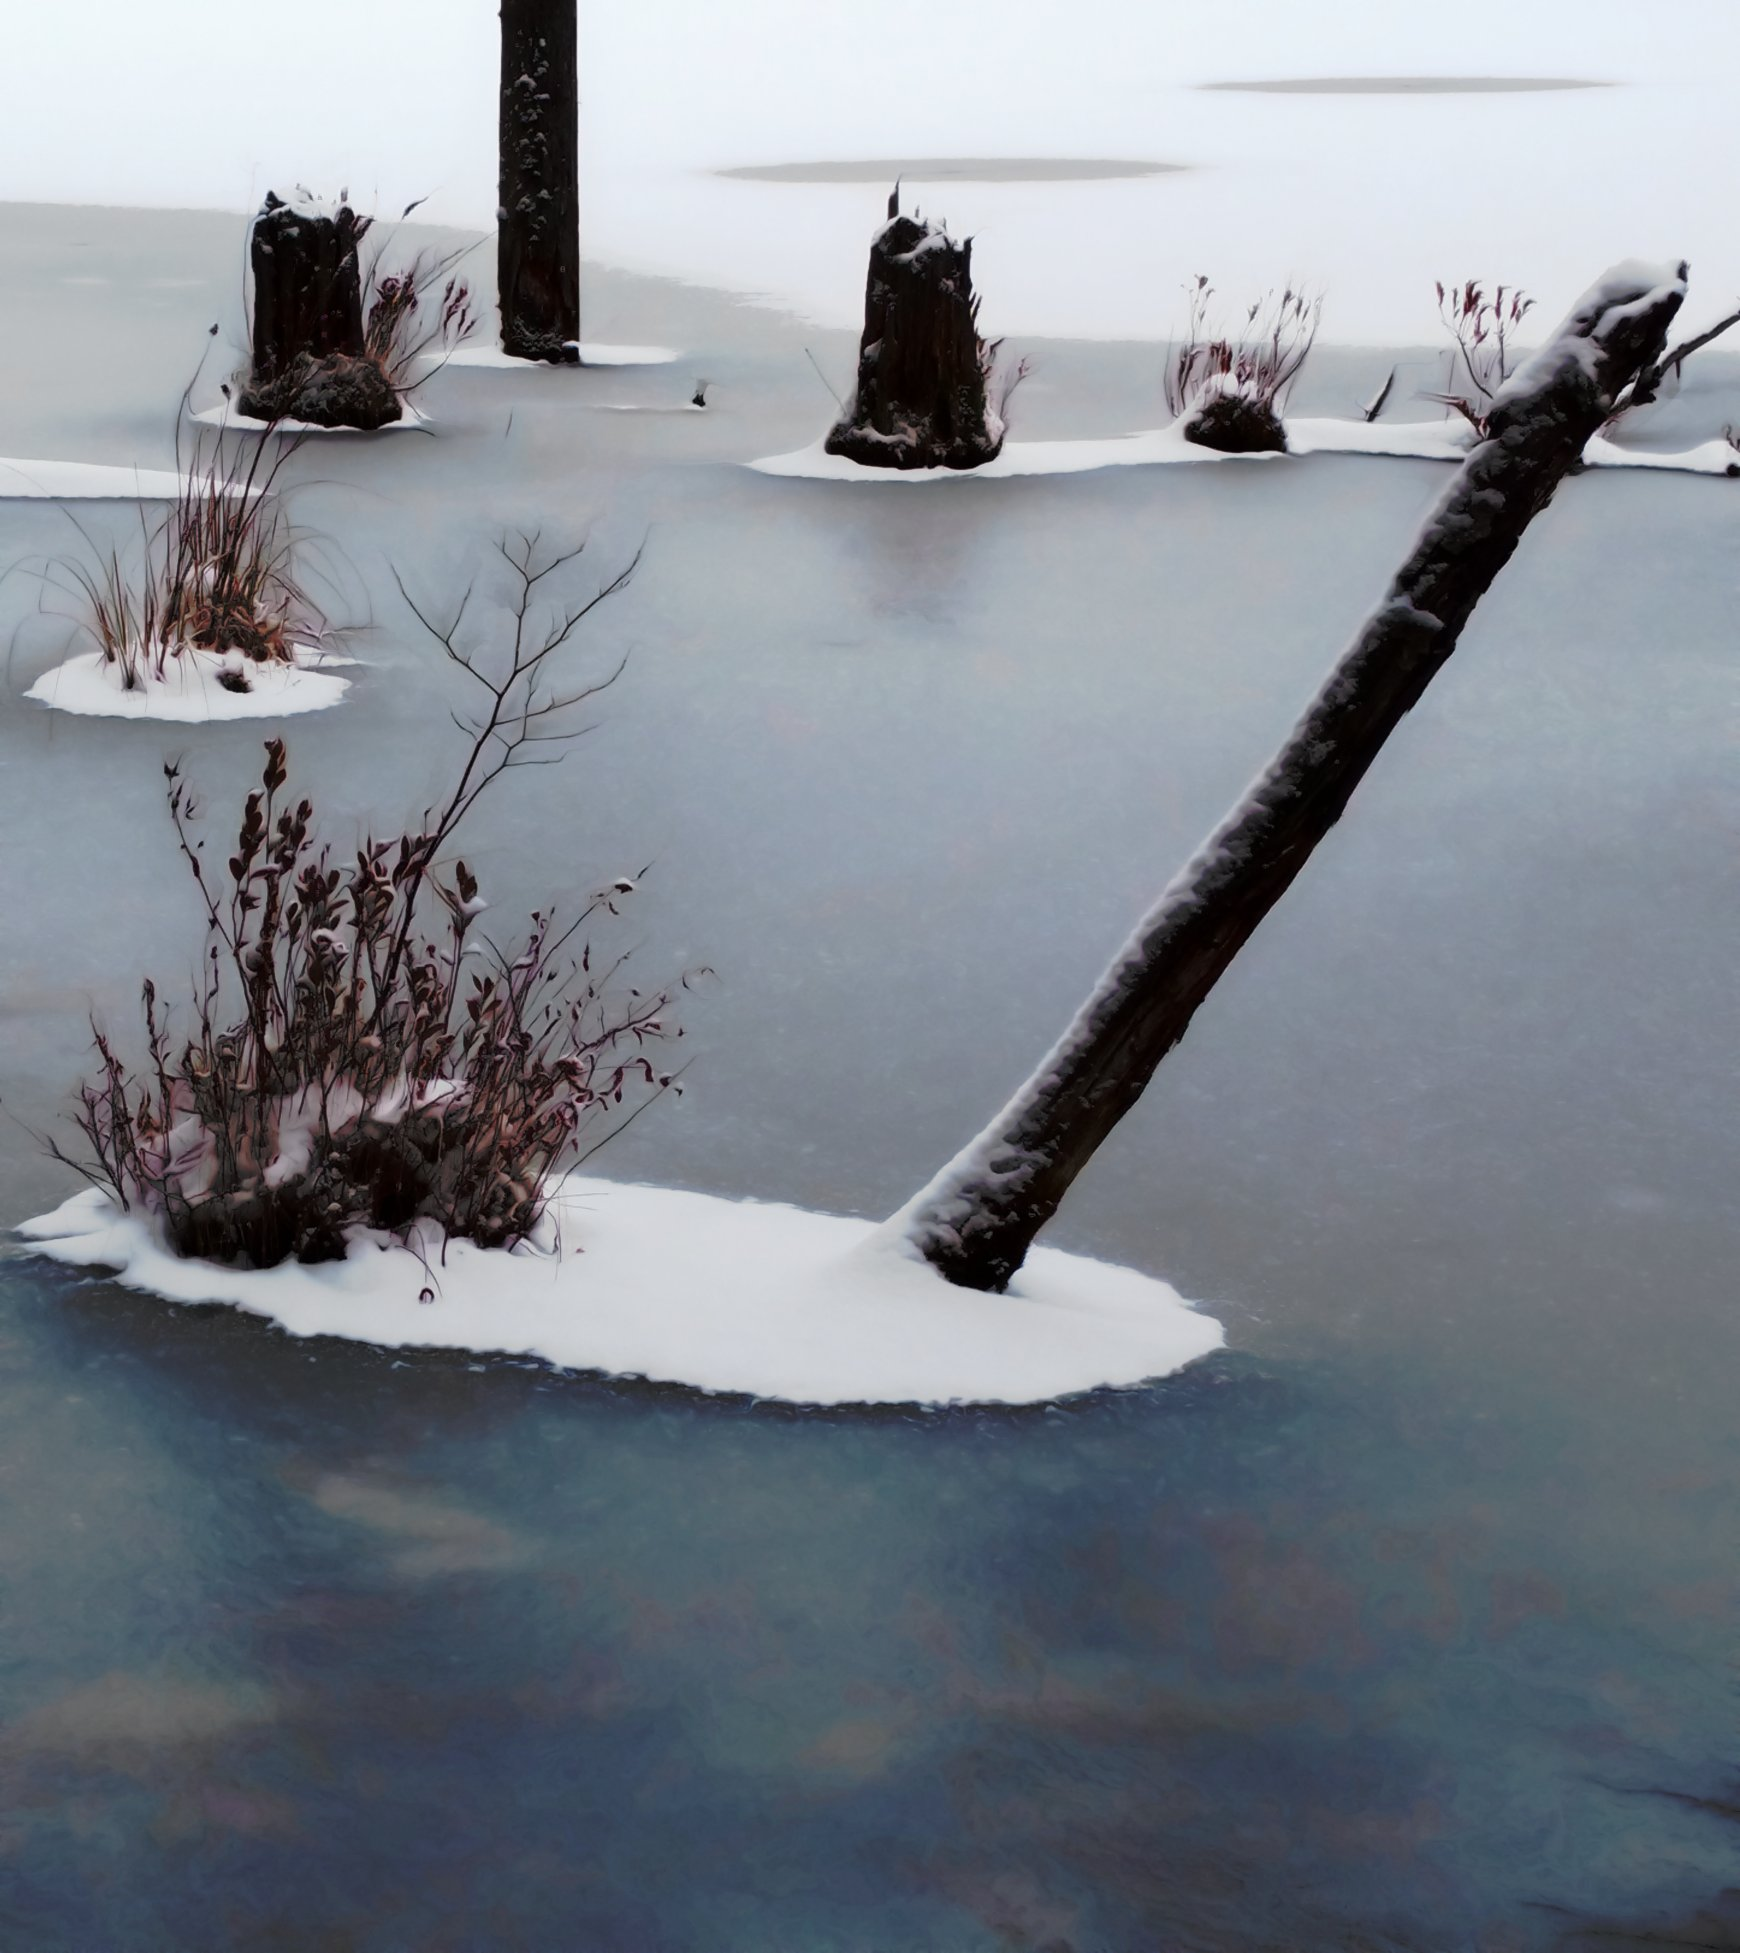
\includegraphics[width=12cm]{img/cover.jpg}

\vspace*{2em}

{\large George W. Matthews}

{\normalsize \cc 2020}

\end{center}

{
\setcounter{tocdepth}{1}
\tableofcontents
}
\hypertarget{preface}{%
\chapter*{Preface}\label{preface}}


\hypertarget{dedication}{%
\section*{Dedication}\label{dedication}}


\begin{centerpic}

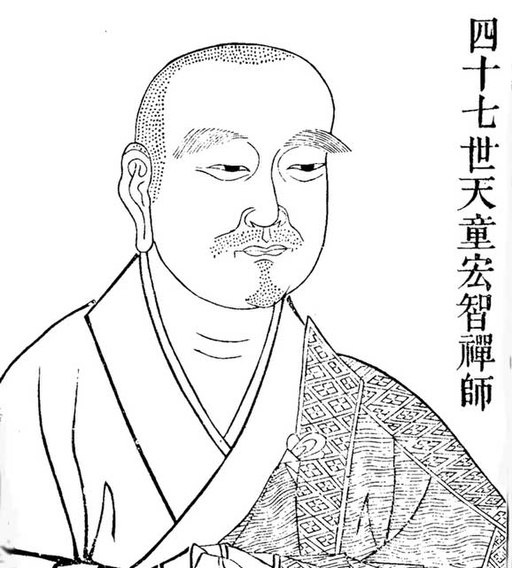
\includegraphics[width=0.4\textwidth,height=\textheight]{img/hongzhi.jpg}

\end{centerpic}

\begin{epigraph}

Receive correctly this monk's word-stream, neither frozen nor trickling away, neither transparent nor muddy. When you wring it dry, take advantage of the opportunity; when you enter the bustle, perceive with your whole eye. Thorough understanding and the changing world fulfill each other totally without obstacle. The moon accompanies the current, the wind bends the grass\ldots Find your seat, wear your robe, and go forward and see for yourself.\\
~\\
---Hongzhi, \emph{Cultivating the Empty Field}

\end{epigraph}

\hypertarget{about-this-book}{%
\section*{About this book}\label{about-this-book}}


\textbf{\emph{May you live in interesting times.}} This is, probably falsely, claimed to be the second worst ancient Chinese curse one might wish upon one's enemies. (The worst one could wish upon them would be ``May you get what you want.'') We, it seems pretty obvious, happen to live in such times, when peace, prosperity, and living to a comfortable if slightly boring old age are no longer as assured as they were even one generation ago. But interesting times are not only unsettled, anxiety provoking times. They are also times full of potential since they force us to call into question previously settled assumptions, and to try to look at things in new ways. Thus they also are times when philosophy flourishes, since philosophy at its best is the relentless and highly focused process of questioning assumptions, making distinctions and seeking solid reasons to back up opinions on the most basic level. Philosophy is the attempt to uncover the truth about the nature of reality, our claims to knowledge and what really matters. If this may seem to be an overly abstract and presumptuous activity when everything is going according to plan, it might become a necessity in times of great social change and stress. Interesting times can force us to examine our assumptions precisely because they starkly reveal the weaknesses in those assumptions. In times such as ours, philosophy becomes more and more urgent. That is part of the motivation for this project.

\textbf{\emph{However,}} it is often the case that philosophy is presented to those new to the field in two ways that discourage the kind of self-examination that interesting times demand of us. It either gets presented as a collection of historical curiosities, to be examined and explicated in ways more suited to historical artifacts than it is to urgent contemporary issues, or it gets smothered in technicalities as if it were of interest exclusively to a small group of people with the time and inclination to learn a highly abstract and specialized vocabulary and a set of microscopically detailed distinctions. Yes historical and textual accuracy is important in describing the development of philosophical thinking in its long and complex history, and yes it is important to be precise and make more and more distinctions to keep on clarifying what exactly we mean. But, it is also important to keep in mind that philosophical questions, methods and conclusions are also always attempts to address pressing human problems. What CAN we really know about things? What IS the nature of our lives, our deaths and what we might hope for? What SHOULD we really be doing with our all too fleeting time here on this planet? And yes, what does it all mean?

\textbf{\emph{This book is an attempt to scratch two itches.}} The first of these is the desire to develop an approach to philosophy that is more directly relevant than other approaches, that shows how philosophical questioning is neither just a historical curiosity, nor a matter only for experts, but is something that makes a difference in our real lives.

\textbf{\emph{The second itch}} I am trying to scratch has to do with initiatives in open education, and I'd like this text to contribute in its own small way to the much larger and more influential open source movement and philosophy of which I consider it a part. Knowledge is only ours to share. Yes of course writers, developers and publishers do hard work that deserves compensation. But intellectual property, it seems to me, is a false idol that deserves to be smashed. So here is my effort to chip away at it -- knowledge should free us and and not sink us into both literal and figurative debt.

\textbf{\emph{In addition}} the decision to place this text into a \href{https://github.com/gwmatthews/philosophy-in-the-wild}{GitHub repository} should be considered as an invitation for others to participate in its future development. Anyone can fork the repository where it resides and use it as a template for their own book project; offer suggestions for revisions, or contribute in other ways as well. Please use the ``issues'' section of the repository for making any major suggestions.

\hypertarget{acknowledgements}{%
\section*{Acknowledgements}\label{acknowledgements}}


\textbf{\emph{The writing}} and publication of this book would not have been possible without the work of numerous people who make and share their amazing work in the open source software community. It is based in particular on the work of \href{https://github.com/yihui}{Yi Hui} and the other developers of \href{https://github.com/rstudio/bookdown}{bookdown} and \href{https://rstudio.com/products/rstudio/}{Rstudio} and related software. While it has been a bit of a steep learning curve figuring out how to use Rstudio and bookdown to write and style a book, it has been a lot of fun too! The end product, hopefully, speaks for itself and demonstrates that these tools are not just for people with highly technical backgrounds, but can be used by anyone with some computer skills and a bit of patience to create functional, cross-platform and pretty good looking web based books.

\begin{center}


\includegraphics[width=0.52083in,height=\textheight]{img/tux.png}

\end{center}

Icons are by Paul Davey, aka \href{http://mattahan.deviantart.com}{Mattahan}. All rights reserved.

\hypertarget{license-cc-by-sa-4.0}{%
\subsection*{License CC BY-SA 4.0}\label{license-cc-by-sa-4.0}}


\textbf{\emph{This book}} is released under a creative commons \href{https://creativecommons.org/licenses/by-sa/4.0/}{CC BY-SA 4.0} license. This means that this book can be reused, remixed, retained, revised and redistributed (including commercially) as long as appropriate credit is given to the authors. If you remix, or modify the original version of this open textbook, you must redistribute all versions of this open textbook under the same license.

\hypertarget{how-to-use-this-book}{%
\section*{How to use this book}\label{how-to-use-this-book}}


\hypertarget{read-it}{%
\subsection*{Read it}\label{read-it}}


This should be self-explanatory, but be sure not to miss the icons on the top of the screen which enable you to:

\begin{itemize}
\tightlist
\item
  Open up and close the sidebar with the table of contents in it.
\item
  Search within the text for a keyword.
\item
  Change the color scheme or font to make it easier to read.
\item
  Offer editorial suggestions on GitHub (see below for how this works).
\item
  Download a pdf version of the text for offline reading or printing.
\item
  Find out keyboard short cuts for navigation.
\end{itemize}

Also note the arrows on the side of the screen (or down at the bottom if you are reading on a small screen) that bring you to the next or previous pages.

\hypertarget{comment-on-it}{%
\subsection*{Comment on it}\label{comment-on-it}}


If you are a current student in one of my Introduction to Philosophy classes you'll have to do some commenting. When I used WordPress to host this text that was a built in feature. Here I am relying on a third party commenting add-on to the online version of the book. There are many ways to do this, with Disqus being one of the most popular. But we won't be using it since they track users and push lots of advertising. Instead we'll be using a nice tool called Hypothes.is, which \protect\hyperlink{appendix-1}{you can find out all about here}.

\hypertarget{contribute}{%
\subsection*{Contribute to it}\label{contribute}}


If you find a mistake, don't think it's clear in some part, have an issue with any part of it, want something more added, etc. I encourage you to contribute. You can do this in a few ways.

\begin{itemize}
\tightlist
\item
  If you have a GitHub account, you can leave a comment in the box at the end of each chapter. That creates an ``issue'' which others can read or add to as well.
\item
  You can also contribute more directly as a pull request by clicking on the ``edit'' button on the top menu bar -- this will take you to the GitHub repository where the source material lives. There you can fork the repository, make whatever edits you want and then offer them in the form of a ``pull request.'' Any such requests will be subject to discussion unless they are minor issues like typos. If you really think I get things all wrong here, fork the book and make it your own! All of this assumes that you:

  \begin{itemize}
  \tightlist
  \item
    Know what ``git'' even is.\footnote{If you don't, it is a version control system that enables collaboration and it mostly intended for software development, but it can be used for working together on any kind of project that involves electronic files, from novels to operating systems.}
  \item
    Have an account at \href{https://github.com/}{GitHub} -- which is free. And \href{https://pages.github.com/}{GitHub pages} is a great way to get yourself a free website too!
  \end{itemize}
\item
  Send me an email if you know me in the real world.
\end{itemize}

\hypertarget{philosophy-and-critical-thinking}{%
\chapter{Philosophy and Critical Thinking}\label{philosophy-and-critical-thinking}}

\hypertarget{what-is-philosophy}{%
\section{What is philosophy?}\label{what-is-philosophy}}

\begin{slideshow}Here is a slideshow summary which can be \href{https://gwmatthews.github.io/philosophy-slideshows/01-phl110-slides.html}{viewed online}, \href{https://gwmatthews.github.io/philosophy-slideshows/pdf/01-phl110-slides.pdf}{downloaded} or \href{https://gwmatthews.github.io/philosophy-slideshows/pdf/01-phl110-handout.pdf}{printed}.

\end{slideshow}

\hypertarget{what-is-a-good-reason}{%
\section{What is a good reason?}\label{what-is-a-good-reason}}

\begin{slideshow}Here is a slideshow summary which can be \href{https://gwmatthews.github.io/ethics-slideshows/02-phl210-slides.html}{viewed online}, \href{https://gwmatthews.github.io/ethics-slideshows/pdf/02-phl210-slides.pdf}{downloaded} or \href{https://gwmatthews.github.io/ethics-slideshows/pdf/02-phl210-handout.pdf}{printed}.

\end{slideshow}

\hypertarget{critical-thinking-toolkit}{%
\section{Critical Thinking Toolkit}\label{critical-thinking-toolkit}}

\begin{slideshow}Here is a slideshow summary which can be \href{https://gwmatthews.github.io/ethics-slideshows/03-phl210-slides.html}{viewed online}, \href{https://gwmatthews.github.io/ethics-slideshows/pdf/03-phl210-slides.pdf}{downloaded} or \href{https://gwmatthews.github.io/ethics-slideshows/pdf/03-phl210-handout.pdf}{printed}.

\end{slideshow}

\textbf{Editorial comments}

If you have a GitHub account and want to make any editorial suggestions, please do so here.

```

\hypertarget{religion-magic-and-metaphysics}{%
\chapter{Religion, Magic and Metaphysics}\label{religion-magic-and-metaphysics}}

\begin{quote}
There are more things in the world than are dreamed of in your philosophy.
\end{quote}

What exactly exists? Is this world of stuff, the natural or material world as studied and further categorized by science, all that there is to reality? Or is the material world just one aspect of reality with other, far less tangible but equally real, domains also part of reality? Are spirits, ghosts, gods, or God real? What about numbers, concepts and other abstract ``things'' -- are they arbitrary symbols for patterns in material things, or do they possess a kind of substance of their own, a reality that is not so much invented by beings capable of grasping abstractions as it is discovered and explored by them?

These are all deep and difficult questions to try to address, and it has been one of the historical preoccupations of philosophers to try to answer them. Doing so has led to the development of a complex and highly technical vocabulary and conceptual apparatus that is often referred to as ``metaphysics,'' or ``ontology.'' But these questions have been central to the project of philosophical self-examination since they have to do with one of the fundamental ways in which our thinking works -- by distinguishing between kinds of things, classifying and categorizing them. This is such a central component of our meaning-making minds that we hardly ever notice it at work. But that it is there and that it is a crucial component of any thinking at all becomes clear when the categories we rely on to make sense of things no longer work as they once did. Fundamental challenges to the basic categories we rely on are somewhat rare, but they do occur from time to time in the lives of individuals, cultures and civilizations.

Take as an example the enormous and persistent backlash against Darwin's theory of evolution that first appeared in Europe and America immediately after the publication of Darwin's great work \emph{On the Origin of Species} in 1859 and continues to this day, more than 150 years later. Darwin's basic theoretical idea, that living organisms on the planet Earth form one big extended family tree that has diversified and changed over time largely through a process called ``natural selection'' is central to the entire field of biology in the same way that atomic theory is central to chemistry, or the way the notions of matter and energy are central to physics. Nothing in biology makes any sense at all with it. And yet, many people outright reject the idea that organisms have evolved over the vast stretches of time that make up the history of life on Earth. And they do so for reasons having to do with the way it challenges fundamental assumptions we have about basic categories -- humans as opposed to animals, blind mechanical and material processes as opposed to intentional and meaningful actions, the animate as opposed to the inanimate.

\hypertarget{being-means-many-things}{%
\section{``Being'' Means Many Things}\label{being-means-many-things}}

\hypertarget{arguing-about-god}{%
\section{Arguing About God}\label{arguing-about-god}}

\hypertarget{magical-thinking}{%
\section{Magical Thinking}\label{magical-thinking}}

\hypertarget{knowledge-science-and-skepticism}{%
\chapter{Knowledge, Science and Skepticism}\label{knowledge-science-and-skepticism}}

\hypertarget{what-can-i-ever-know}{%
\section{What Can I Ever Know?}\label{what-can-i-ever-know}}

\hypertarget{science-or-superstition}{%
\section{Science or Superstition?}\label{science-or-superstition}}

\hypertarget{knowing-what-isnt-so-cognitive-biases.}{%
\section{Knowing What Isn't So: Cognitive Biases.}\label{knowing-what-isnt-so-cognitive-biases.}}

\hypertarget{minds-machines-and-freedom}{%
\chapter{Minds, Machines and Freedom}\label{minds-machines-and-freedom}}

\hypertarget{minds-and-bodies}{%
\section{Minds and Bodies}\label{minds-and-bodies}}

\hypertarget{thinking-machines}{%
\section{Thinking Machines?}\label{thinking-machines}}

\hypertarget{causes-effects-and-freedom}{%
\section{Causes, Effects and Freedom}\label{causes-effects-and-freedom}}

\hypertarget{ethics}{%
\chapter{Ethics}\label{ethics}}

\hypertarget{culture-religion-and-morality}{%
\section{Culture, Religion and Morality}\label{culture-religion-and-morality}}

\hypertarget{when-push-comes-to-shove-relativism-in-theory-and-practice}{%
\subsection{When Push Comes to Shove: relativism in Theory and Practice}\label{when-push-comes-to-shove-relativism-in-theory-and-practice}}

\hypertarget{religion-and-the-question-of-foundations}{%
\subsection{Religion and the Question of Foundations}\label{religion-and-the-question-of-foundations}}

\hypertarget{cultural-universals}{%
\subsection{Cultural Universals?}\label{cultural-universals}}

\hypertarget{whats-in-it-for-me}{%
\section{What's in it For Me?}\label{whats-in-it-for-me}}

\hypertarget{psychological-egoism}{%
\subsection{Psychological Egoism}\label{psychological-egoism}}

\hypertarget{in-defense-of-capitalism}{%
\subsection{In Defense of Capitalism}\label{in-defense-of-capitalism}}

\hypertarget{self-other-and-ethics}{%
\subsection{Self, Other and Ethics}\label{self-other-and-ethics}}

\hypertarget{expanding-the-circle}{%
\section{Expanding the Circle}\label{expanding-the-circle}}

\hypertarget{the-common-good}{%
\subsection{The Common Good}\label{the-common-good}}

\hypertarget{human-rights-the-universal-realized}{%
\subsection{Human Rights: The Universal Realized}\label{human-rights-the-universal-realized}}

\hypertarget{expanding-the-horizon}{%
\subsection{Expanding the Horizon}\label{expanding-the-horizon}}

\hypertarget{social-and-political-philosophy}{%
\chapter{Social and Political Philosophy}\label{social-and-political-philosophy}}

\hypertarget{the-social-contract}{%
\section{The Social Contract}\label{the-social-contract}}

\hypertarget{on-the-orgins-of-society}{%
\subsection{On the Orgins of Society}\label{on-the-orgins-of-society}}

\hypertarget{markets-and-morals}{%
\subsection{Markets and Morals}\label{markets-and-morals}}

\hypertarget{just-deserts}{%
\subsection{Just Deserts}\label{just-deserts}}

\hypertarget{self-and-other}{%
\section{Self and Other}\label{self-and-other}}

\hypertarget{racism-and-fear-of-the-other}{%
\subsection{Racism and Fear of the Other}\label{racism-and-fear-of-the-other}}

\hypertarget{gender-sexuality-identity}{%
\subsection{Gender, Sexuality, Identity}\label{gender-sexuality-identity}}

\hypertarget{imaginary-homelands}{%
\subsection{Imaginary Homelands}\label{imaginary-homelands}}

\hypertarget{art-philosophy-and-meaning}{%
\chapter{Art, Philosophy and Meaning}\label{art-philosophy-and-meaning}}

\hypertarget{meaning-form-expression}{%
\section{Meaning, Form, Expression}\label{meaning-form-expression}}

\hypertarget{new-worlds-and-ways-of-seeing}{%
\section{New Worlds and Ways of Seeing}\label{new-worlds-and-ways-of-seeing}}

\hypertarget{representation-and-social-conflict}{%
\section{Representation and Social Conflict}\label{representation-and-social-conflict}}

\hypertarget{how-to-write-a-chapter}{%
\chapter{How to Write a Chapter}\label{how-to-write-a-chapter}}

\begin{centerpic}


\includegraphics[width=0.5\textwidth,height=\textheight]{img/construction.png}

\begin{centercap}

figure caption

\end{centercap}

\end{centerpic}

\begin{epigraph}

Pithy epigraph.\\
~\\
---Wise Person

\end{epigraph}

\begin{center}

\begin{argument}

This is a template for writers of chapters. Each chapter consists of a single page like this and has three to five subsections. Open up the file 99-Template.Rmd and save it as a copy to create a new page. Then just replace this text with your own and follow the models for formatting images text boxes links and more.

\end{argument}

\end{center}

\textbf{\emph{Opening words of sentence}} gets highlighted and everything else is normal.

\hypertarget{summary}{%
\section*{Summary}\label{summary}}


This is an embedded html slideshow. It is an iframe embed and so in principle anything could fit here. Have a look at the css to see the format trick for adjusting proportion to different media. Here the css class is ``slideshow.'' Compare that class to the ``video'' class -- the principle is the same.

\begin{slideshow}Here is a slideshow summary which can be \href{https://gwmatthews.github.io/ethics-slideshows/01-slides.html}{viewed online}, \href{https://gwmatthews.github.io/ethics-slideshows/pdf/01-slides.pdf}{downloaded} or \href{https://gwmatthews.github.io/ethics-slideshows/pdf/01-handout.pdf}{printed}.

\end{slideshow}

\hypertarget{further-exploration}{%
\section*{Further exploration}\label{further-exploration}}


\begin{itemize}
\tightlist
\item
  Michael Sandel is a philosophy professor at Harvard who teaches a very popular course called ``Justice'' that explores material that overlaps with this text. His extensive website \href{http://justiceharvard.org/}{Justice with Michael Sandel} also has videos of his lectures from that course the first of which focuses on the famous runaway trolley example.
\end{itemize}

\end{document}
